% first example chapter
% @author Jan Robert Rösler 
%
\chapter{Idee}

\section{DroNet und Carolo-Cup}

\paragraph{DroNet}
Die \gls{gl:eth} entwickelte 2018 eine eigene Architektur, mit dem Ziel durch Training auf Fahrbahnbildern eine Drone zu steuern \cite{Loquercio_2018}. 
Das daraus entstandene, von Aufbau und Größe relativ einfach gehaltene Neuronale Netz, war der Anstoß für diese Arbeit. 

Das Netz, in seinem Aufbau dargestellt in Abbildung~\ref{img:DroNet}, bekommt als Input ein 200x200 Pixel großes Bild in Graustufen, der Output ist ein Lenkwinkel und zusätzlich eine Kollisionswahrscheinlichkeit.

\begin{figure}[h]
	\centering
	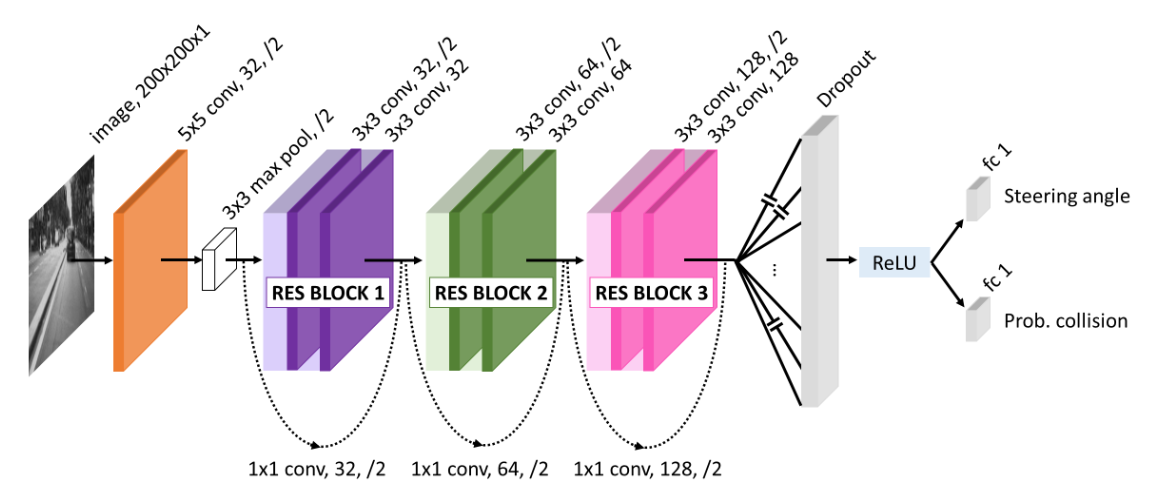
\includegraphics[scale=0.5]{figures/Architecture-DRONET.png}
	\caption{Architektur \textsc{DroNet}}
	\label{img:DroNet}
\end{figure}

Trainiert wurde das Netz auf frei verfügbaren Datensätzen der Firma \gls{gl:udacity}, bestehend aus Bildern aufgenommen mit Kameras hinter der Windschutzscheibe eines Autos bei stundenlagen Fahrten über Amerikanische Highways. Die Aufnahmen sind mit Fahrdaten verbunden, Zeitstempel, GPS-Daten, Beschleunigungswerte und Lenkwinkel wurden für jedes Bild der Aufnahmen gespeichtert. Für das Training von \textsc{\gls{gl:dronet}} werden nur die Bilder der Mittelkamera und der jeweilige Lenkwinkel genutzt.

Zusätzlich hat das Team der ETH Zürich eigene Aufnahmen mithilfe einer am einem Fahrrad montierten Kamera im Straßenverkehr gemacht und diese Aufnahmen manuell mit einer Kollisionswahrscheinlichkeit versehen. Wie bereits erwähnt hat das Netzwerk dementsprechend zwei verschiedene Outputs.\\
Für diese Arbeit ist aber nur der Lenkwinkel von Interesse, Kollision spielt als Szenario keine Rolle. Im Entwurf werden dementsprechend Anpassungen gemacht.

Es stellte sich heraus, dass das Modell der ETH Zürich hervorragend generalisierte und eine Drohne sicher durch ein Straßenszenario steuern konnte, wobei das Szenario sich deutlich von den gelernten Unterschied. Diese Eigenschaft von \textsc{DroNet} möchte ich mir im folgenden zu Nutze machen und auf dieser Basis ein Steuerungsmodell für ein RC-Fahrzeug entwickeln.

\paragraph{Carolo-Cup}
Die \gls{gl:haw} nimmt seit einigen Jahren am \glqq \gls{gl:carolo} \grqq{} teil, einem Wettbewerb der Technischen Universität Braunschweig. Hier treten Teams einiger deutscher Hochschulen mit RC-Fahrzeugen (Maßstab 1:10) in verschiedenen Disziplinen des autonomen Fahrens gegeneinander an. Der Wettbewerb findet jährlich in Braunschweig auf einem vorbereiteten Kurs statt.

Eine hauptsächlich von den HAW Studenten Nils Schönherr und Gunnar Wolfram aufgebaute Plattform, zu sehen in Abbildung~\ref{img:Carolo-Fahrzeug}, dient dieser Arbeit als Testplattform.

\begin{figure}[h]
	\centering
	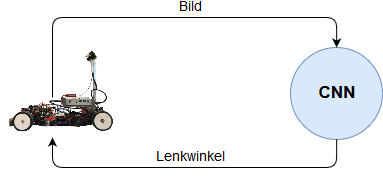
\includegraphics[scale=0.7]{figures/Aufbau.png}
	\caption{Einfacher schematischer Aufbau }
	\label{img:Aufbau}
\end{figure}


Zum Entwickeln der Fahrzeuge steht an der HAW eine Teststrecke zur Verfügung, verschiedene Fahrzeugplattformen sind in der Entwicklung.\\
Vor diesem Hintergrund entstand die Idee für diese Arbeit.

\paragraph{Ziel}
Das Ziel dieser Bachelorarbeit ist, an einem konkreten Anwendungsfall zu zeigen, dass ein Fahrzeug autonom einen Streckenkurs abfahren kann, indem ein neuronales Netz live Bilder der Strecke auswertet und Lenkinformationen für das Fahrzeug berechnet, schematisch dargestellt in Abbildung~(\ref{img:Aufbau}). Da aktive Teams der HAW im Carolo-Cup aktuell klassische (Bildbasierte-) Navigationsansätze verfolgen (Kapitel~\ref{sec:Autonome Navigation mit Bilddaten}), soll die Arbeit auch zeigen, wie eine nächste Generation der Fahralgorithmen für den Carolo-Cup aussehen kann.

Die autonome Fahrleistung auf der Teststrecke ist das Hauptaugenmerk, sie zu messen und zu analysieren ist Bestandteil der Arbeit.



